%%%%%
\section{Integration among different databases}\label{sec:integsurvey}
In this section we're interested to attack the \textbf{multi-database integration} problem, that can be stated as follows: \textit{given a global schema $G$ of my integrated system and a query\index{query|textbf} $q$ written in a  \textsc{Language} $\langg_G$, evaluate such query among multiple data-sources $\mathcal{D}=\Set{D_1,\dots, D_n}$ having   different schemas and data representations}. This definition is general enough to include both distributed and federated databases data integration.

In order to proficiently solve this problem, we're going to see that ontologies (Section \ref{sec:ontology}), generalizing data schemas  \cite{GangemiP13}, allow to attack the schema matching problem (Section \ref{subsec:ontaling}) on different data sources with several schemas and representations. Last, the problem of evaluating query $q$ on either the original data sources or on the global schema will be addressed (Section \ref{subsec:queryrw}).


%As a consequence, we have first to reconcile the ontology describing each database $D_i\in\mathcal{D}$ with the global ontology $G$. We will always use ontology matching instead of schema matching because both it has been showed that ontologies are more general than data models \cite{GangemiP13}, and because

\subsection{Preliminaries: Description Logic and Ontologies}\label{sec:ontology}
When compared with other data models such as the three world relational model for data mining \cite{Calders2006}, MOF\index{MetaObject Facility} also shows its inability to outline and suggest which are the relevant operations to either manipulate the data or to perform assertions on it. Ontologies are now introduced in particular for the latter reason, thus allowing to assert properties on the required by the \textsc{Model} level, and \textit{objects} and \textit{relations} at the \textsc{Data} level. The following generic definition of an ontology is provided in literature:

\begin{definition}
	\label{def:taonta}
	An \textbf{ontology}\index{ontology|textbf} \cite{Allemang2011} is a semantic interpretation of a model establishing relations among model's types and defining generic inference rules. Moreover ``\textit{an ontology plays a role of a semantic domain in denotational semantics}'' \cite{saeki} and refers to concepts or entities, that are language  and representation independent \cite{mathmeta}.
\end{definition}

Even though the MOF characterization clearly puts the ontology at the \textsc{Language} level, the unclear literature characterization has the problem of distinguishing \textsc{Model}s$\index{M}$ from ontologies \cite{terrasse} because their distinction is ``\textit{diverse and frequently contradictory}'' \cite{mathmeta}. On the other hand, other researchers cited in \cite{saeki} claim that the aim of distinguishing \textsc{Model}s from ontologies is to separate the representation of the information from the description of the data collected inside it. On the other hand, \cite{saeki} distinguishes the \textsc{Model} from the ontology level by defining a semantic mapping function associating each element of the \textsc{Model} to a collection of the elements of the ontology. Within the MOF characterization, such definition matches with the $\alpha$ function, where each element of the ontology is provided within one single formula predicating the properties associated to the type.

Among all the possible classes of  \textsc{Language} expressing ontologies (such as \textbf{frame-based} or \textbf{first order logic-based} languages \cite{Corcho00}), we chose to  describe ontologies using Description Logic (DL)\index{description logic} languages. This choice is due to the wide diffusion of OWL, a member of the DL language family, for Semantic Web applications. DL is also widely dealt in current literature, such that their notation is even adopted for expressing generic concepts in data integration literature \cite{euzenat2013d}. As a consequence, we provide a DL-biased definition for an ontology:

\begin{definition}[Description Logic Ontology]\label{def:dlonta}
	Given a set $I=\Set{i_1,\dots,i_n,\dots}$ of individuals, a \textbf{description logic ontology} $O$ \index{ontology!description logic} \index{description logic|see {ontology}} is a pair $(\mathcal{A},\mathcal{T})$, where both properties of individuals and binary relations between such individuals are expressed.

In particular, $\mathcal{A}$ is called \textbf{ABox} because it contains the following types of term, called \textbf{axioms}:
	\[t_{\mathcal{A}}:=C(i)\;|\;R(i,i')\;|\;C_1\sqsubseteq C_2\;|\;C_1\equiv C_2\;|\;R_1\sqsubseteq R_2\;|\; R_1\equiv R_2\]
	where $C$ describe \textbf{concepts} (\textit{types}) characterizing the individuals, and $R$ represent \textbf{roles} (\textit{relationships}) among source ($i$) and destination ($i'$) individuals. Moreover, inclusions ($\sqsubseteq$) and equivalence ($\equiv$) between the concepts could be also defined among concepts or roles.

$\mathcal{T}$ represents the \textbf{TBox} containing all the assertions and properties concerning the statements within the ABox. Such assertions are expressed within description logic languages, which expressive power and computational complexity may vary depending on the constructors of choice. An example of such constructors for the SROIQ language is provided in Table \ref{tab:SROIQ}.
\end{definition}

As a consequence, the \textsc{Model} is a part of the ontology ($M_O$) describing the collection of all the types that could be represented. On the other hand, ABox and TBox statements do not allow to transform individuals into others via transcoding functions $\transcoding$, because such logic focuses more on expressing properties over existing data than on showing which operations shall be used on top of such data.

\begin{table}
\centering
	\begin{tabular}{l|l|ll}
	\toprule
	& Description & Syntax ($\cdot$) & Semantics ($\cdot^{\mathcal{I}}$)\\
	\midrule
%\textbf{Individuals} 	& & \\
%individual name &	$o$ &	$o^{\mathcal{I}} = o$ \textbf{s.t.} $o\in D_O$\\
\parbox[t]{2mm}{\multirow{3}{*}{\rotatebox[origin=c]{90}{\textbf{Roles}}}} & atomic role &  $R$ & $\{r\in D_R|\alpha(r)=R\}$ \\
& inverse role & $R^{-}$ & $\{(x,y)|(y,x)\in R^{\mathcal{I}}\}$\\
& universal role & $U$ & 	$D_O\times D_O$\\
\midrule
\parbox[t]{2mm}{\multirow{11}{*}{\rotatebox[origin=c]{90}{\textbf{Concepts}}}} & atomic concept & $A$ & $\{o\in D_O| \alpha(o)=A\}$\\
& intersection &	$C\sqcap D$ & $C^{\mathcal{I}}\cap D^{\mathcal{I}}$\\
& union &	$C\sqcup D$ & $C^{\mathcal{I}}\cup D^{\mathcal{I}}$\\
& complement &	$\neg C$ & $D_O\backslash C^{\mathcal{I}}$\\
& top & $\top$ & $D_O$\\
& bottom & $\bot$ & $\emptyset$ \\
& existential restriction 	& $\exists R. C$ & $\{o\in D_O|  \exists o'\in D_O. (o,o')\in R^{\mathcal{I}} \wedge o'\in C^{\mathcal{I}}\}$ 	\\
& universal restriction 	& $\forall R. C$ & $\{o\in D_O|  \forall o'\in D_O. (o,o')\in R^{\mathcal{I}} \Rightarrow o'\in C^{\mathcal{I}}\}$ 	\\
& at-least restriction & $\geq n\; R.C$ & $\Set{o\in D_O|\left|\Set{o'\in D_O|(o,o')\in R^{\mathcal{I}}\wedge o'\in C^{\mathcal{I}}}\right|\geq n }$ \\
& at-most restriction & $\leq n\; R.C$ & $\Set{o\in D_O|\left|\Set{o'\in D_O|(o,o')\in R^{\mathcal{I}}\wedge o'\in C^{\mathcal{I}}}\right|\leq n }$ \\
& reflexivity & $\exists R. \textsc{Self}$ & $\Set{x\in D_O| (x,x)\in R^{\mathcal{I}}}$\\
& nominal & $\{o\}$ & $\{o|o\in D_O\}$\\
\bottomrule
	\end{tabular}
	\caption{Syntax and semantics of SROIQ constructors using \textsc{Data} as a domain for the interpretation under the CWA. SROIQ is the DL language expressing the OWL2.}
	\label{tab:SROIQ}
	\end{table}


Another difference between Description Logic and standard query  \textsc{Language} is that the preferred TBox interpretation  relies on the ``open world assumption'' (OWA)\index{OWA} \cite{Baader2010}. This implies that the truth value of the DL statements may be true irrespectively of whether or not it is known to be true within the ABox, thus opposing their query interpretation to the closed world assumption (CWA)\index{CWA}, where only the represented data are assumed to be true, thus describing a ``negation as failure'' approach (NAF, \cite{REN2010692}). As a consequence,  OWA semantics for {very expressive languages leads to an undecidable evaluation of the TBox assertions, thus preventing to use such languages for practical interests} \cite{baader2017}. On the other hand, the axiomatic restrictions of the CWA lead to decidable evaluations of DL languages \cite{PatelSch12}, albeit still intractable in some cases. Within the CWA assumption where the \textsc{Data} layer as the domain of the interpretation for both individuals and roles, and assuming that each individual is an actual object of the \textsc{Model}$\index{M}$ level, $C(i)$ could be interpreted as $\abstr(i)=C$. Please also note that, while MOF allows the representation of a multigraph, thus allowing multiple edges between two vertices, the description logic does not permit to refer to one specific edge among a given source and destination. This last observation makes the standard DL characterization unserviceable on top of our data model, thus requiring to extend such language.

Still within the field of Modal Logics but beyond DL languages\footnote{DL could be considered as a class of languages providing extensions to modal logic.}, the Register Logic language \cite{Barcelo2013} makes  constraint checking tractable at the price of the loss of expressive power of graph navigation, but allowing to execute queries always in data polynomial time (\textsc{NLogspace}).



\subsection{Ontology Alignments and Data Integration}\label{subsec:ontaling}
After describing an ontology, we're going to use ontology alignments for attacking the data integration problem. Such class of solutions have received more research acclaim than schema related one \cite{Magnani09,Magnani2010}, which are strictly representation dependent.

%In order to introduce and explain this problem, an example is going to be provided. 
At this point we must extend the Description Logic syntax so that individual transformation functions $\stigma$ are allowed, in order to be able to express supertypes'\index{supertype} transcoding functions. Such transformations will be required in the following scenario in order to say that  $C(i)\sqsubseteq C'(\transcoding(i))$. %\hl{Last, this example introduces for the first time in the field of ontology alignment the concept of ontologies' relationships alignment, when such relationships occur within a same source ontology}.


%{\color{red}in order to make the definition possible which is independent from the semantics of the given data, despite several attempts of providing ontologies a structure \cite[Chapter~5,~page~221]{Baader2010}.}

%There have been some data modeling approaches similar to the ones of the MetaObject Facility and the UML standard \cite{Pan01,Brasileiro2016}, thus failing to represent ontology as reasoning tools, and hence as (query) languages over which express properties of the data (\textsc{Model} and \textsc{MetaModel}) and the \textsc{Data} itself. \texttt{[TODO]} This requires that the syntactic representations in the (meta-)model layer should be linked with their semantic counterparts in the (meta-)ontology:
% TODO:
%Ontologies could be used to point out different points of view over the same subject {\color{blue} Inserire in questo punto il concetto di allineamento delle ontologie.} \cite{small,somewhere}; ontologies are also useful {\color{red}for giving predictions by using inference tools: this is possible since ontologies are described in a language (e.\,g.\, Description Logic) that has a formal and logic-based semantic and that have also decision procedures that  make automated reasoning possible}.

After describing in the previous sections how ontological alignments are useful within the process of data integration, we can now formally define what an alignment between two ontology is. Moreover, since in some scenarios the alignment uses the data representation to infer such alignment \cite{Aligon201520}, I extend the usual alignment definition provided for either schema or ontology alignments \cite{euzenat2013d,GrossHKR11} as follows:

%%%%%%%%%%%%%%%%%%%%%%%%%%%%%%%%%%%%%%%%%%%%%%%%%%%%%%%%%%%%%%%%%%%%%%%%%%%%%%%%%
%
%\subsection{(Meta-)Modelling, Modelling Language and Type Theory}
%Let us start by analysing data modelling independently from the usage of a specific given modelling language. As a start, works like \cite{terrasse,saeki} and even the theoretical formulation in \cite{mathmeta} do not use the meta-meta-model, and terminate their abstraction at the meta-model level, since such meta-meta-model could be easily be replaced by a meta-model \cite{UMLInfra}. The abstraction process could be used to define the layers, since states that each layer is the result of applying steps of abstraction.
%
%
%

%
%%\begin{figure}
%%	\centering
%%	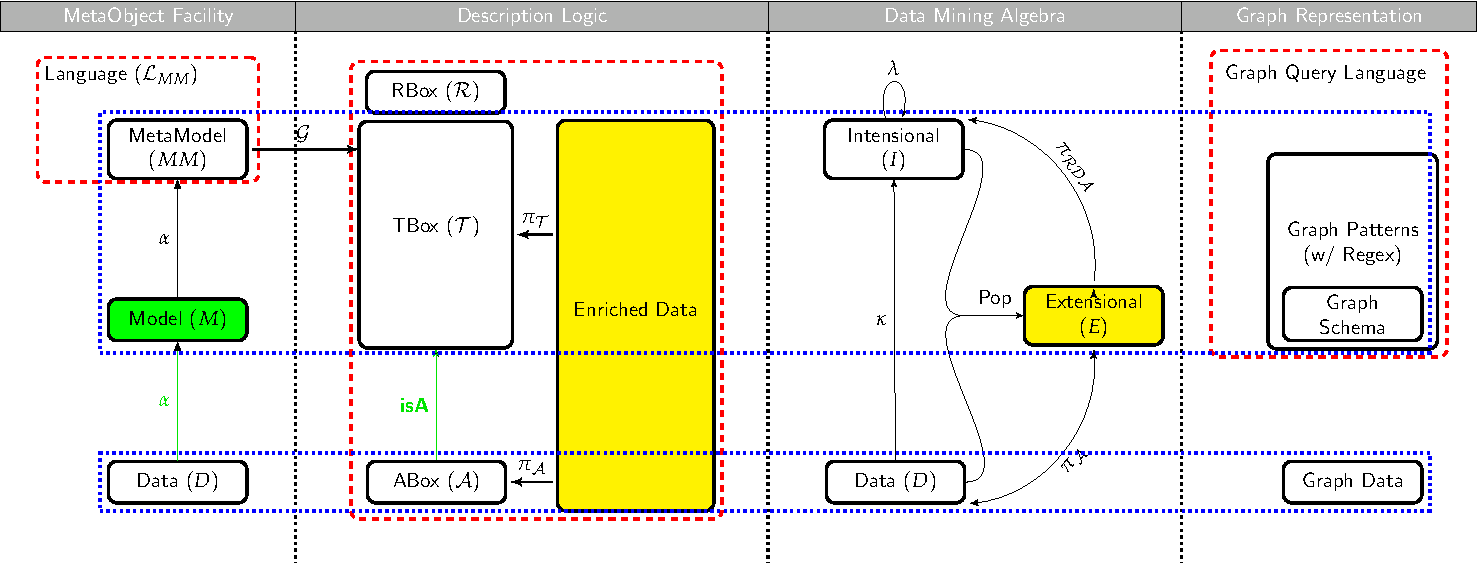
\includegraphics[width=\textwidth]{images/taonta}
%%	\caption{Data modeling using different approaches: structuded data representation dependent (\textit{MetaObject Facility} \cite{omg96}), representation independent and language driven (\textit{Description Logic} \cite{Calvanese2010}), structured data representation dependent and language driven (\textit{Data Mining Algebra} \cite{Calders2006}), semistructured data representation dependent (\textit{Graph Representation}).}
%%	\label{fig:taonta}
%%\end{figure}

\begin{definition}[Ontological Alignment]\label{def:ontolalignment}
An \textbf{ontological alignment}\index{alignment|textbf}  $\alignment(O,O')$ of a source ontology $O$ towards a destination ontology $O'$ is a set of tuples called \textbf{correspondences}\index{correspondence|textbf}. Each correspondence %refers to a type $T$ belonging to the model $M_{O'}$ associated to the destination ontology $O'$. 
maps a set of types $\delta t$ from a model $M_O$ into one type $t$ in $M_{O'}$ using a transcoding \index{transcoding} function $\stigma_{\delta t\to t}$ mapping elements in $\delta t$ to $t$.
Such correspondence is expressed as $(\delta t,F,t,\transcoding_{\delta t\to t}, s)$, where $F$ is the alignment expressed in description logic axioms between the correspondent types and, %$\stigma_{\mathcal{P}(M_O)\to T}$ is the function transforming the data $\alpha^{-1}(\delta\mathcal{T})$ into $T$ and, 
whenever $\transcoding_{\delta t\to t}$ is a bijection\footnote{If $t$ expresses a \textbf{part-of} or an \textbf{is-a} relation such as $\delta t\sqsubseteq t$, then sometimes is not possible to univocally associate to the aggregation the single disaggregated components.}, the inverse function $\transcoding_{ t\to \delta t} = \transcoding_{\delta t\to t}^{-1}$ is also provided. An uncertainty score $s$ could be also associated to the accuracy of the alignment \cite{euzenat2013d,HartungGR13}.
\end{definition}

As a consequence of this definition, given that the ontology subsumes both the informations from the \textsc{Model}$\index{M}$ (it describes the concepts and roles) and the ones from the \textsc{MetaModel}$\index{MM}$ (TBox expressions), we have that a  \textsc{Language} $\langg_\metamodel$ could be also described by the language expressed in its correspondent ontology. %$\mathcal{G}(\alpha^{-1}(MM))$, and hence $\mathcal{L}_{MM}\equiv \mathcal{L}_{\mathcal{G}(\alpha^{-1}(MM))}$. 
%As a consequence, from now on we'll talk about languages for ontologies.
 In the case of Description Logic Ontologies, the query  \textsc{Language} is the Description Logic itself. Given that both ontologies (containing the schema definition, $\metamodel$) and queries could always be expressed within the Description Logic (\cite[Chapter~16]{Baader2010}), from now on we'll always use the terms \textit{query}\index{query}, \textit{ontology}\index{ontology} and \textit{schema}\index{schema} interchangeably as already did in \cite{Lenzerini02}.




%
%Figure \ref{fig:taonta} finally provides a global point of view on layers and
%their relations: $\alpha$ provides abstractions in order to reach meta-levels,
%while $\alpha_1$ and $\alpha_2$ are to be interpreted as projection functions,
%where only data or ontologies are grasped from an enriched context.
%
%As \cite{kleppe} suggests, we need to find a formalism through which express
%data, models and meta-models. We are also interested in defining transforming
%function among those, that is defining different semantic interpretations of
%the same initial concept \cite{saeki}.
%Since we want to make data and model translation possible, we would
%like to express our data relations and structural modification with a modelling language
%that is not necessarily a .
%
%
%By the way the definition of XMI suggests us that it is possible to describe
%the $D$, $M$ and $MM$ layer in the same language representation. Hence
%we want to use a language where we could
%express not only relations between data and models and meta-models, but also
%to express data and model transformations. In order to reach this aim, we have
%to use a system where we could represent data and define queries and transformations
%over it. We would also like to define data transformations over models in the
%same language.


%The latter definition also includes the definition of a \textit{(binary) data integration system} \cite{Lenzerini02} and generalizes it, by replacing schemas with ontologies as in \cite{DeGiacomo2018} and by replacing one-way mappings with more general ontology alignmnets, where $O$ assumes the role of the \textbf{local} ontology representing the local data sources, and $O'$ represents the \textbf{global} ontology, which is the target of the whole alignment process.
%
%\begin{definition}[Binary Data Integration System]
%	A \textbf{binary data integration system} is defined as a triple $I=\Braket{G,L,A(G,L)}$, where $G$ is the global ontology, representing the target of the alignment process, $L$ is the local ontology, representing the local data sources, and $A$ is an ontological alignment (Definition \ref{def:ontolalignment}).
%\end{definition}
As outlined by both more recent literature \cite{GrossHKR11,HartungGR13} and  in the former Example, it is possible to provide alignments between multiple local ontologies into one single global ontology, which in this case it is referred as \textit{hub (ontology)}. Therefore, the previous definition could be extended as follows:

\begin{definition}[Multisource Data Integration System]
	\index{data integration!multisource}
	A \textbf{multisource data integration system} is defined as a triplet $\Braket{H,\mathcal{I},\mathcal{O}}$, where $H$$\index{H|textbf}$ is the \textit{hub} ontology\index{ontology!hub|see{$H$}}, representing the target of all the  ontological alignments  $A(O,H)\in\mathcal{I}$ having $O\in\mathcal{O}$ as a source (or local) ontology.
\end{definition}
